\pagebreak
\subsection{Mechanical Design} \label{Mechanical_Design}

 \begin{figure}[H]
     \centering
     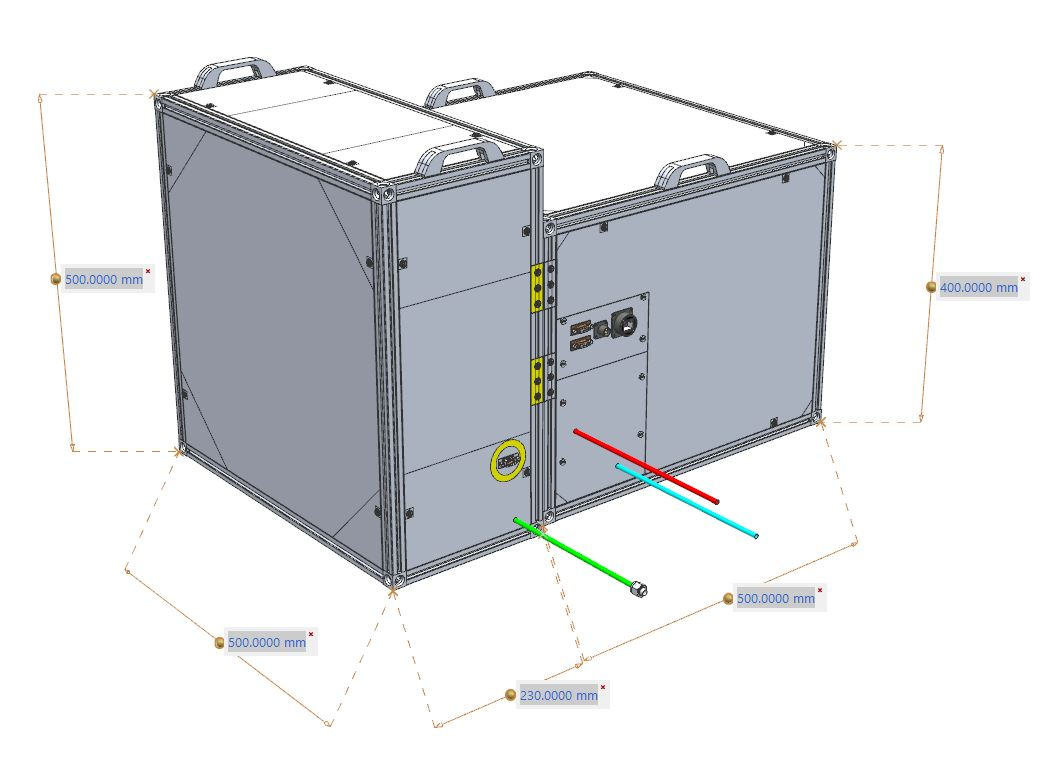
\includegraphics[width=1\textwidth]{4-experiment-design/img/Mechanical/tubular_dimensions.jpg}
     \caption{General Dimensions of the Experiment.}
     \label{dimensions}
\end{figure}

\begin{table}[H]
\noindent\makebox[\columnwidth]{%
\scalebox{0.8}{
\begin{tabular}{c|c|c|c|}
\cline{2-4}
 & CAC & AAC & TOTAL \\ \hline
\multicolumn{1}{|c|}{Experiment mass {[}kg{]}} & $12.08$ & $12.37$ & $24.45$ \\ \hline
\multicolumn{1}{|c|}{Experiment dimensions {[}m{]}} & $0.23\times0.5\times0.5$ & $0.5\times0.5\times0.4$ & $0.73\times0.5\times0.5$ \\ \hline
\multicolumn{1}{|c|}{Experiment footprint area {[}m^2{]}} & $0.115$ & $0.25$ & $0.365$ \\ \hline
\multicolumn{1}{|c|}{Experiment volume {[}m^3{]}} & $0.0575$ & $0.1$ & $0.1575$ \\ \hline
\multicolumn{1}{|c|}{Experiment expected COG position} & \begin{tabular}[c]{@{}l@{}}$X=23.51\ cm$\\ $Y=10\ cm$\\ $Z=22.57\ cm$ \end{tabular}  & \begin{tabular}[c]{@{}l@{}} $X=29.04\ cm$\\ $Y=16.63\ cm$\\  $Z=16.2\ cm$ \end{tabular} &\begin{tabular}[c]{@{}l@{}} $X=26.31\ cm$\\ $Y=24.99\ cm$\\  $Z=19.35\ cm$  \end{tabular} \\ \hline
\end{tabular}}}
\caption{Experiment Summary Table.}
\label{table:experiment-summary}
\end{table}


As it is mentioned in Table \ref{table:experiment-summary}, the Center Of Gravity for the whole experiment appears to be located just on base of the third level of The Brain which coincides with the location of the electronics PCB. This outcome is quite advantageous in terms of stability for one of the most sensitive subsystems of the experiment in terms of shakes and loads. Notice that the values for the center of gravity are based on the reference axis shown in Figure \ref{COG}. Also, the table weights of the boxes and, therefore, the whole experiment, are increased by a $10\%$ of safety margin.

 \begin{figure}[H]
     \centering
     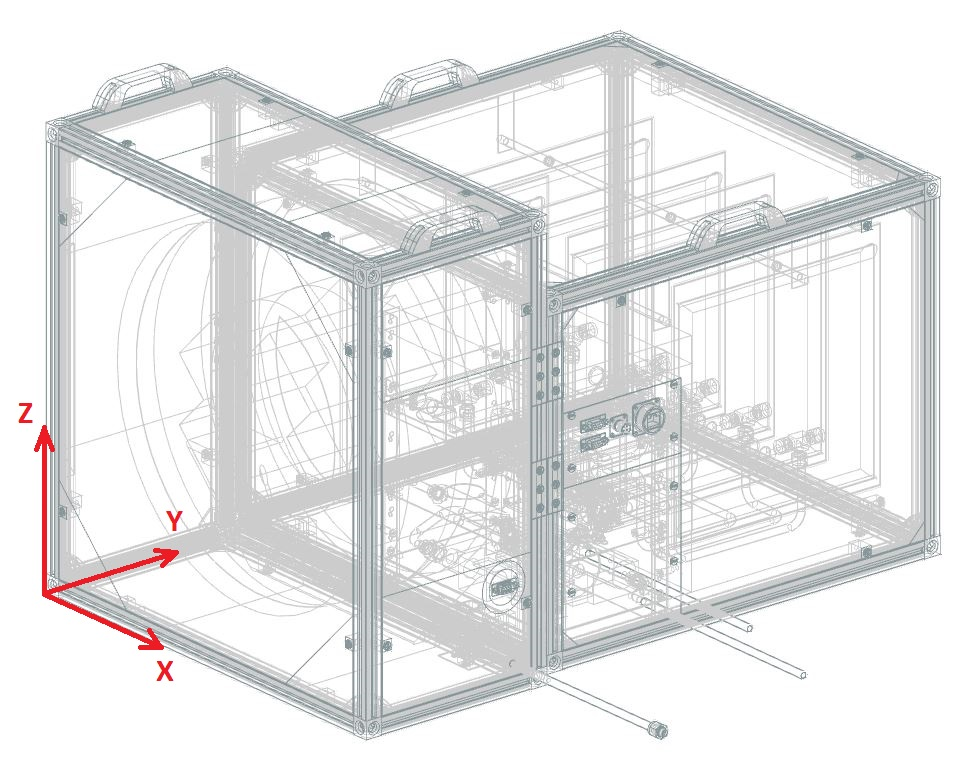
\includegraphics[width=0.7\textwidth]{4-experiment-design/img/Mechanical/COG.jpg}
     \caption{Reference Axis for the Total Center of Gravity.}
     \label{COG}
\end{figure}

\subsubsection{Structure}
\label{sec:4.4.1}

The experiment consists of two rectangular boxes, one stacked next to the other. The higher but narrower box - CAC box - allocates the heaviest element, the CAC. The main box - AAC box - contains the AAC system as well as the central command unit: The Brain. The Brain contains the general Electronic box (EB) as well as the pneumatic sampling system. The frame of these two boxes will be made of aluminum bars which have a characteristic cross-section of 20x20 mm. The rails will allow an easy interface between bars and other elements.

% % Figure of 3 bars

 \begin{figure}[H]
     \centering
     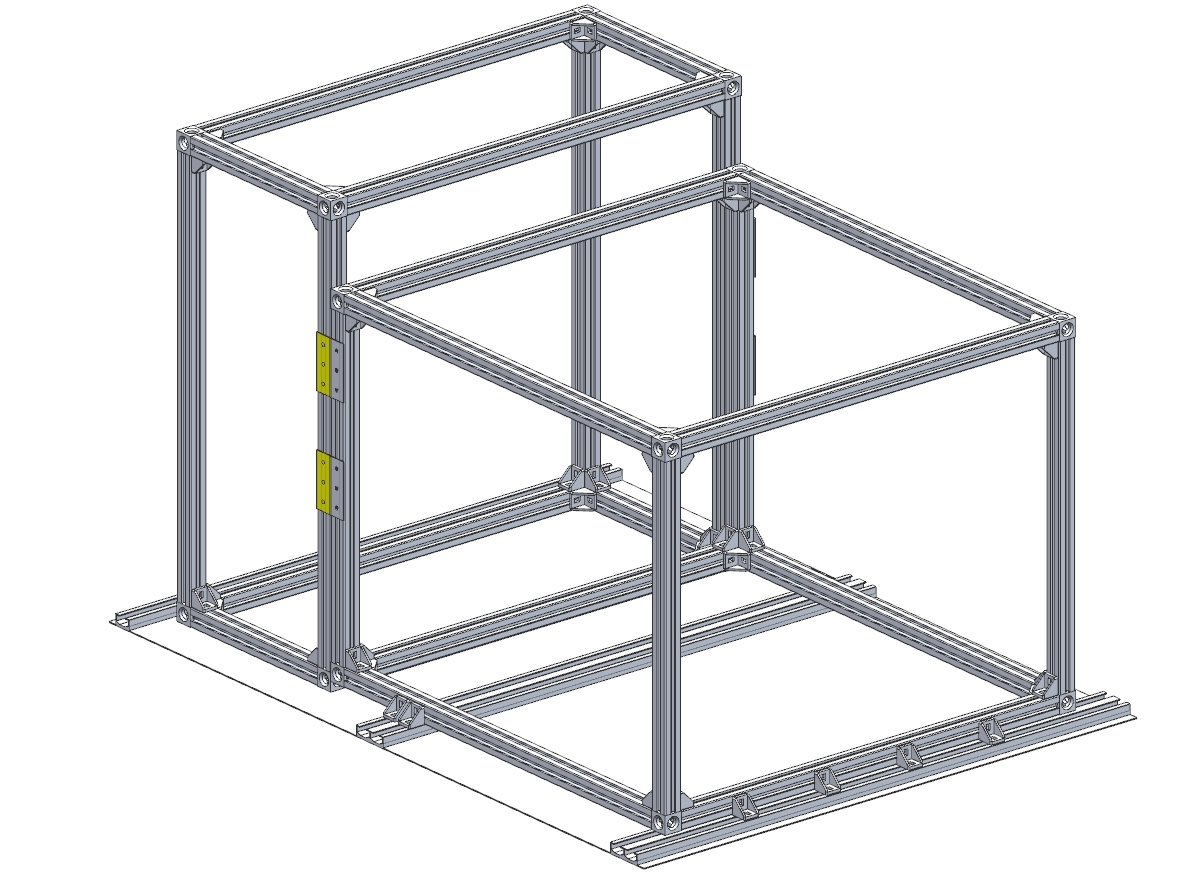
\includegraphics[width=0.9\textwidth]{4-experiment-design/img/Mechanical/structure_pic.jpg}
     \caption{Structure Overview.}
     \label{structure}
\end{figure}

The frame is designed to withstand all vibrations and ensure a reliable stability of the entire system. Test 9 in Table \ref{tab:vibration-test} will help to confirm the frame can withstand these vibrations and updates to the design will be made if necessary. 

The frame of the structure, shown in Figure \ref{structure}, is built by the aforesaid aluminum strut profiles which are connected to each other with cubic connectors 20/3 that provide better strength and stability for the whole structure. These two components are connected by M6x16 normalized bolts aligned with the bars axis. At the same time, these nodes will be reinforced by three brackets (see Figure \ref{fig:bracket}) each.

Table \ref{table:materials_prop} shows the main properties of the materials used to manufacture the main structural components.




\begin{longtable}{|m{0.1\textwidth}| m{0.3\textwidth} |m{0.14\textwidth} |m{0.16\textwidth}|m{0.13\textwidth}| m{0.14\textwidth} |}
\hline
Material & Application & Density & Tensile strength & Yield Strength & Modulus of elasticity  & Brinell hardness \\ \hline 
Aluminium 5754 & Wall sheets,  brain structure plates, CAC-AAC join plate & $2.67 g/cm^3$ & $190 MPa$ & $80 MPa$ & $70 GPa$ & $77 HB$ \\ \hline
Aluminium 6105-T5 & Strut profiles & $2.7g/cm^3$ & $310 MPa$ & $275MPa$ & $69 GPa$ & $95 HB$ \\ \hline

\caption{Main structural materials.}
\label{table:materials_prop}
\end{longtable}
\raggedbottom




The two-box design will allow ease of access and manipulation of both the CAC and AAC subsystems, see Figure \ref{fig:3D_tubular_render}. In addition, the AAC sampling system is designed to be re-usable for future handover to FMI, as such, it will be mountable on any standard balloon flight without having to introduce major design changes. The latter would mean to introducing a battery as a power unit, hence less bags could be carried (around five bags) in this potential future setup, see Figure \ref{battery_distribution}.

% Figure of the two structures
%\begin{figure}[!ht]
%    \centering
%    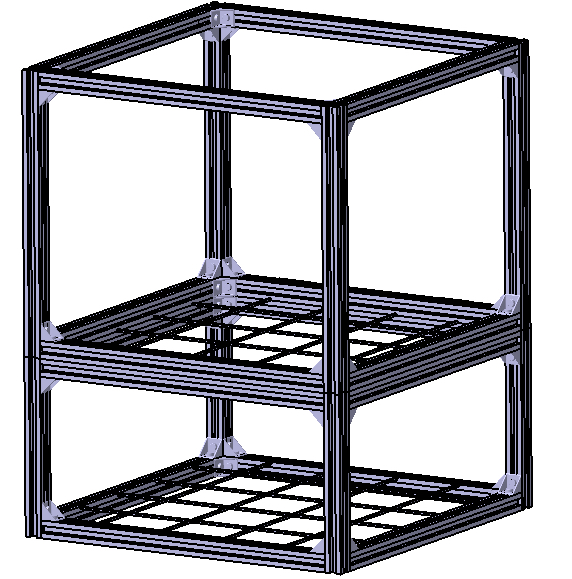
\includegraphics[width=0.7\textwidth, angle=90]{4-experiment-design/img/frame_structure.jpg}
%    \caption{Structure of the two-box design.}
%    \label{strucutre}
%\end{figure}



\pagebreak
\subsubsection{CAC Subsystem}

The CAC subsystem is designed to fit a 300 m stainless steel coiled tube, a solenoid valve governing it, interfaces, an air filter and three temperature sensors. A schematic of this subsystem can be seen in Figure \ref{fig:CAC-schematic}. The CAC consists in a combination of a 200 m coiled tube of 1/8 in. and a 100 m coiled tube of 1/4 in. The outlet of the CAC is sealed with a quick connector provided by FMI. The inlet will be sealed in the same way but it will be open by means of another interfaced plugged to the quick connector. A filter is placed between this orifice and the solenoid valve. The filter will be custom made by FMI. The set up is a tube containing magnesium perchlorate powder with stone wool at both ends of the tube. It will ensure that no moisture will enter the coil during any testing or sampling. Another tube is attached to the solenoid valve that goes outside the box, thus having a direct outside outlet and inlet for the whole CAC system, as seen in Figure \ref{fig:CAC-cad-model}.

\smallskip
The electronic components in the CAC box will be: three temperature sensors and the solenoid valve. In order to connect to these components, a male D-sub connector will be placed at a position on the wall of the box, where it is shortest distance to the EB in the AAC box (third level of The Brain). A female D-sub connector will also be placed on that wall of the AAC box. The connection between these plugs is made through a D-Sub wire. 
% mechanical issues and gondola constraints 

\begin{figure}[H]
    \centering
    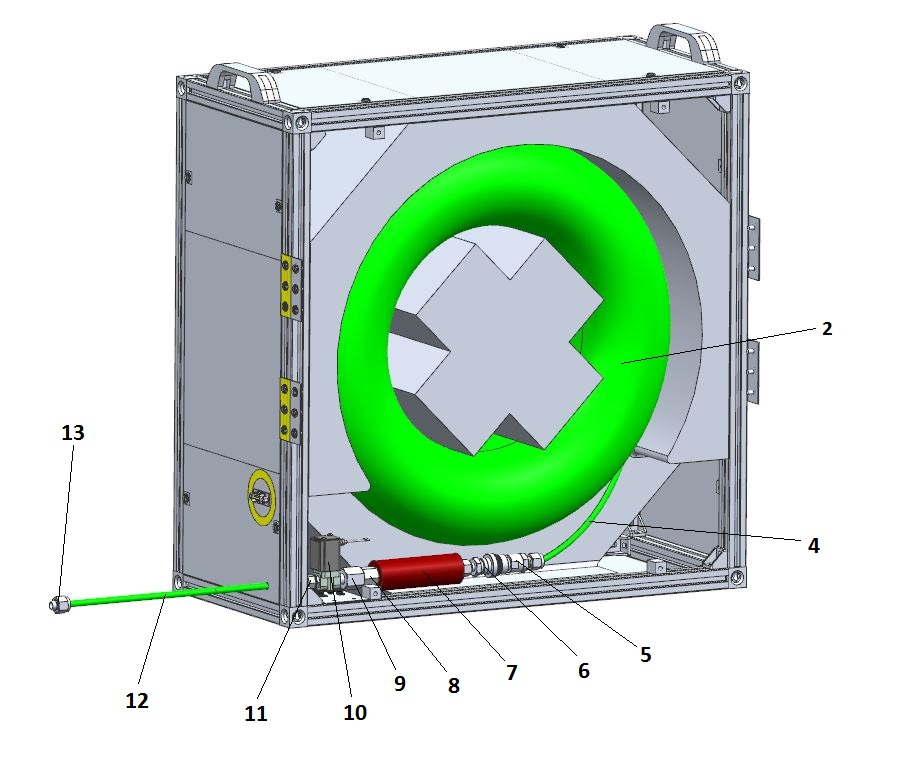
\includegraphics[width=0.8\textwidth]{4-experiment-design/img/Mechanical/CAC_interior_labels.jpg}
    \caption{3D Model of the CAC Box. The Numbers Correspond to the Numbers in Figure \ref{fig:CAC-schematic}.}
    \label{fig:CAC-cad-model}
\end{figure}

\begin{figure}[H]
    \centering
    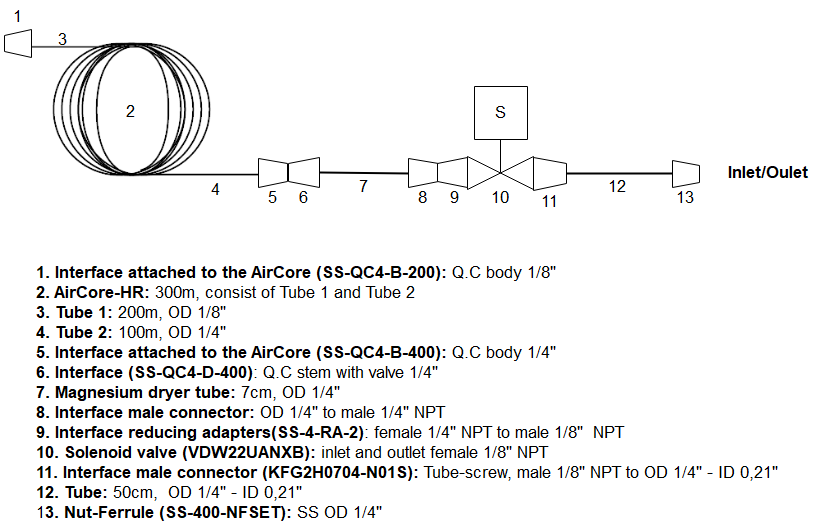
\includegraphics[width=1\textwidth]{4-experiment-design/img/CAC-schematic-v3.PNG}
    \caption{Schematic of CAC}
    \label{fig:CAC-schematic}
\end{figure}

Since the CAC will be the heaviest component in the whole experiment, its positioning and orientation inside the gondola will directly affect the stress analysis of the structure, hence it must be considered.

\smallskip
Firstly, it is possible to identify the interface to attach the experiment box to the gondola as one of the most critical points in terms of mechanics performance. In the worst case scenario, with a heavy experiment and without a proper study of the aforesaid interface, shear in the screws could be produced after a violent landing stress or unexpected shaking. The larger the distance to the fixed points, the bigger the momentum produced by the component. Nevertheless, due to fast recovery implementation, the CAC tube will be placed vertically. Therefore, its dedicated box will be properly attached to the AAC box by means of four anchor points, fast recovery fixing interface as seen in yellow in Figure \ref{dimensions}. The fast recovery then will only imply unscrewing 12 screws and unplugging a D-Sub connector. 


\pagebreak
\subsubsection{AAC Subsystem}\label{sec:aac-analysis}

The AAC Subsystem consists of six 3 L sampling bags. Each bag will have a dedicated valve in the Valve Center (VC) to allow emptying and filling processes as well as to close the bag when needed. The bags will be placed vertically and will have two anchor points: on the top through a  multiple anchor interface (see Figure \ref{anchor_bags}) and on the bottom by means of the tubes connecting them to the valves.

%% Several Figures of the top box with its inside elements: isometric, top view and front view.

\begin{figure}[H]
    \centering
    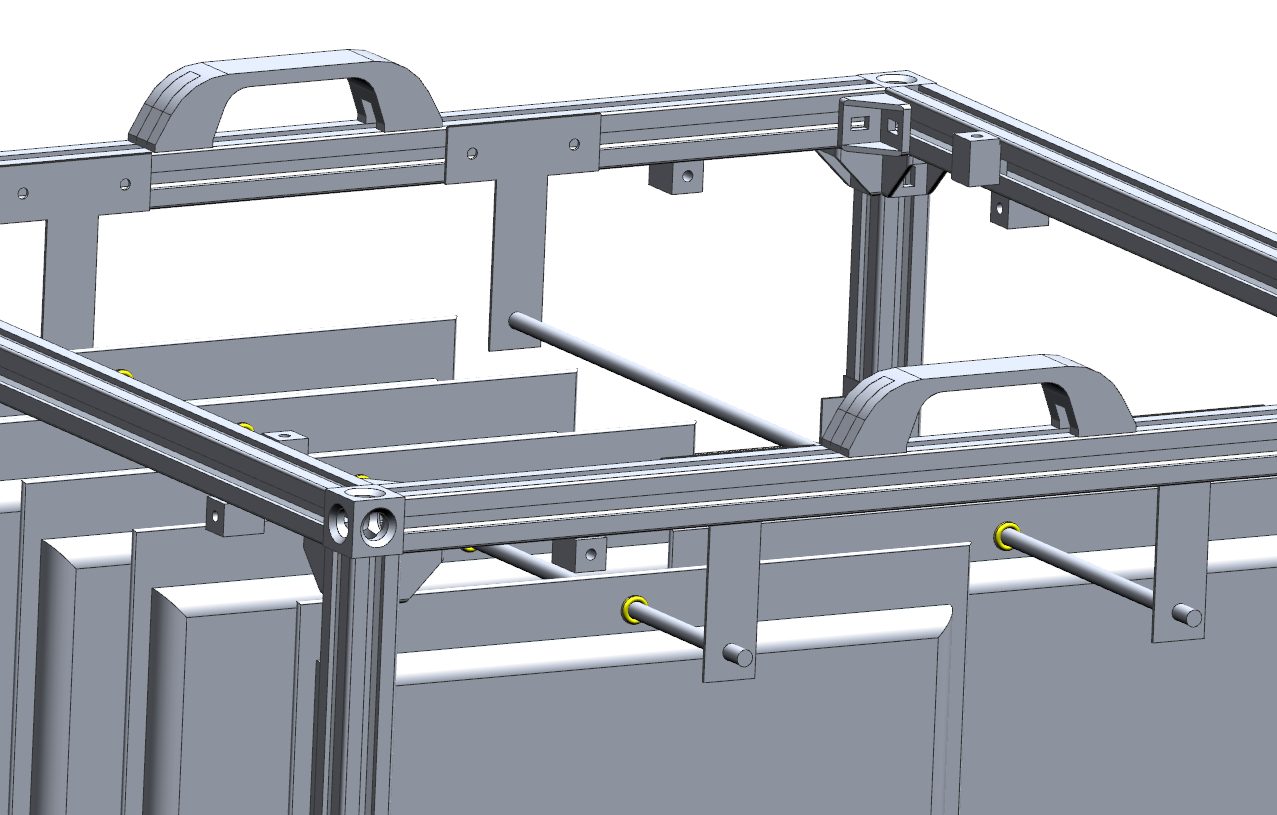
\includegraphics[width=0.7\textwidth]{4-experiment-design/img/Mechanical/Bags_Fixing_Interface.png}
    \caption{Sampling Bags with Fixing Interface and the AAC Box Handles.}
    \label{anchor_bags}
\end{figure}

Table \ref{table:bags-dimensions} shows how the dimensions of the bags change according to the sampled volume. This data has been obtained by testing and has been taken into account in order to determine the maximum number of bags that can be filled inside the box.

\begin{table}[H]
\noindent\makebox[\columnwidth]{%
\scalebox{0.8}{
\begin{tabular}{|c|c|c|c|}
\hline
\textbf{Volume} & \textbf{Length (horizontal)}& \textbf{Height (vertical)} & \textbf{Width }\\ \hline
Empty & 26.4 cm & 28 cm & 0.5 cm \\ \hline
0.5 L & 26.4 cm & 27.5 cm & 1.5 cm \\ \hline
1 L & 26 cm & 27.5 cm & 2 cm \\ \hline
1.5 L & 25.5 cm & 26.5 cm & 4.5 cm \\ \hline
2 L & 25 cm & 25 cm & 5.5 cm \\ \hline
2.5 L & 24.5 cm & 23 cm & 7.5 cm \\ \hline
3 L & 24 cm & 22 cm & 10.5 cm \\ \hline
\end{tabular}}}
\caption{Dimensions of the Bags When Filled with Different Air Sample Volumes}
\label{table:bags-dimensions}
\end{table}

\pagebreak
\underline{Distribution}

The AAC box has been designed in order to be as compact as possible. Nonetheless, the latter was a challenging iterative process since the bags dimensions vary during the flight. The process led to a square base box that is able to fit six sampling bags together with a control center called The Brain that includes the pneumatic system and the electronic box. The distribution layout can be seen in Figures \ref{iso_aac} and \ref{lateral_aac}.

% Figure: Top view to show the distribution of the AAC Box

\begin{figure}[H]
    \centering
    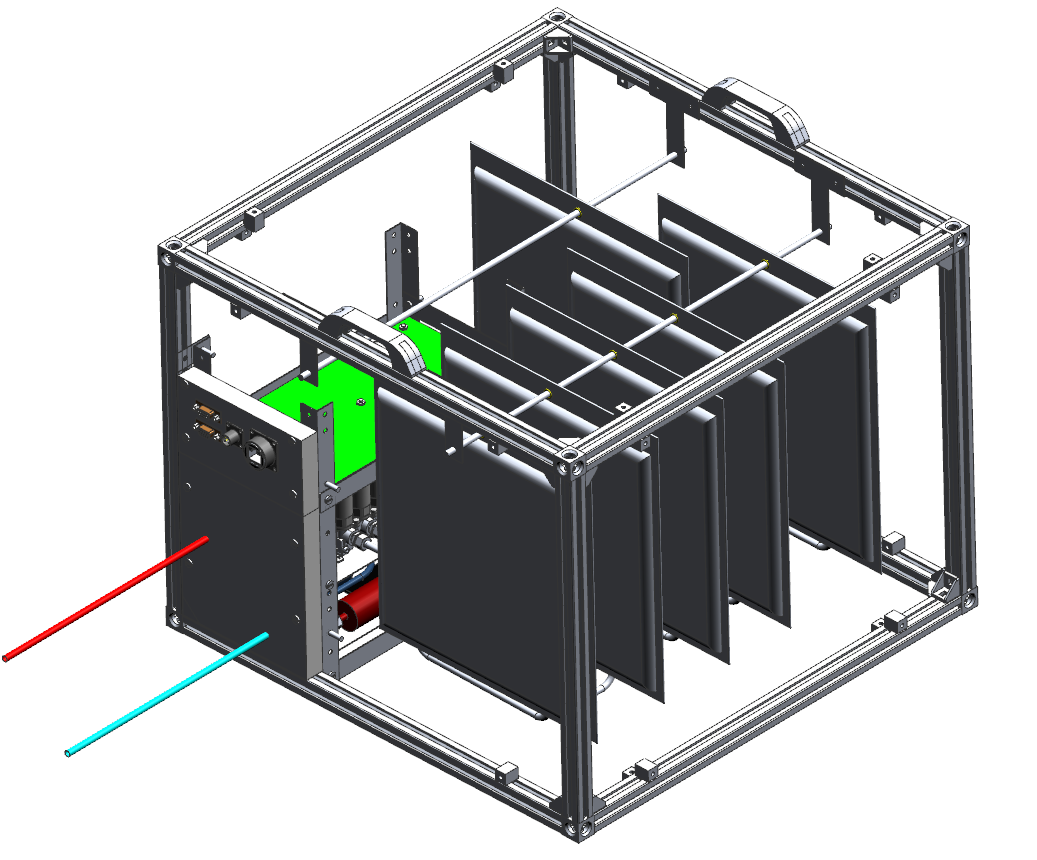
\includegraphics[width=0.8\textwidth]{4-experiment-design/img/Mechanical/AAC_isometric_view.png}
    \caption{Isometric View of the AAC Box.}
    \label{iso_aac}
\end{figure}


\begin{figure}[H]
    \centering
    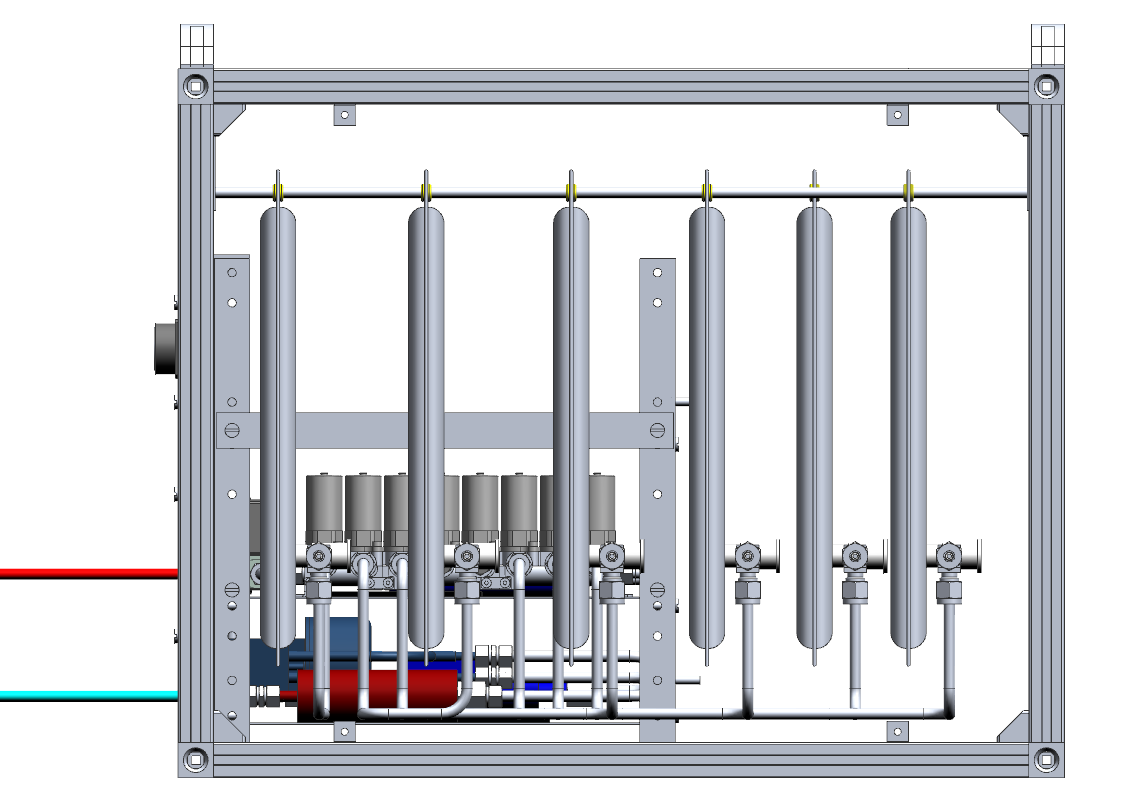
\includegraphics[width=0.8\textwidth]{4-experiment-design/img/Mechanical/AAC_lateral_view.png}
    \caption{Lateral View of the AAC Box.}
    \label{lateral_aac}
\end{figure}

\begin{figure}[H]
    \centering
    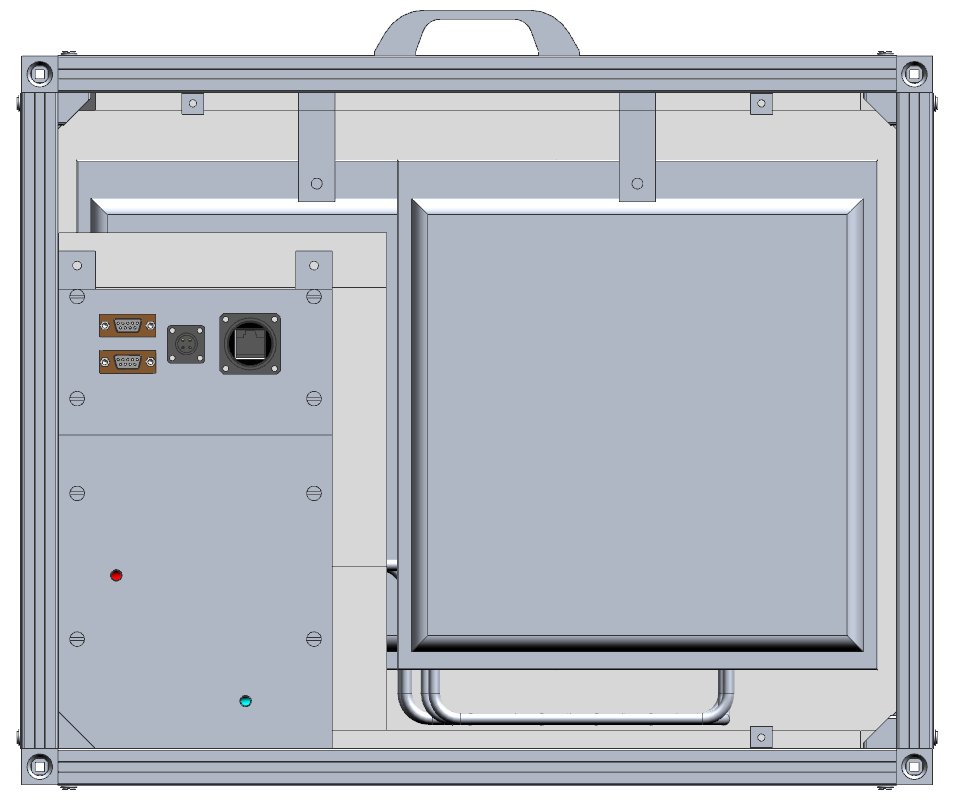
\includegraphics[width=0.8\textwidth]{4-experiment-design/img/Mechanical/AAC_front_view.png}
    \caption{Front View of the AAC Box.}
    \label{front_aac}
\end{figure}

In order to reach to all the bags from the Valve Center, the tubes are brought to the base of the box. More detail on its positioning is included in the following section. 

\smallskip
Since the AAC box is expected to be handed over to FMI, the design also takes into consideration the possibility to include a battery for power supply. This would be allocated next to the Brain. The latter would imply reducing the sampling bags down to five, see Figure \ref{battery_distribution}.

% Figure with a a top view without the 6th bag and with a red box simulating the battery

\begin{figure}[H]
    \centering
    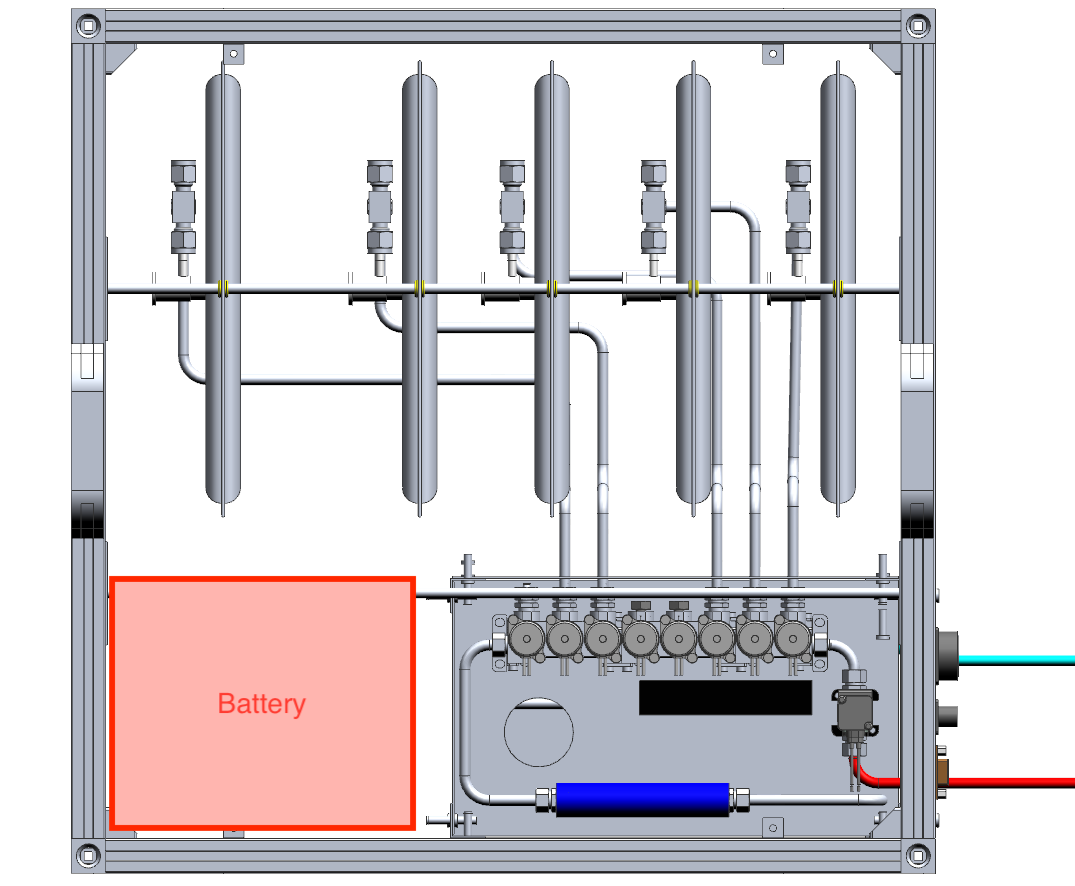
\includegraphics[width=0.8\textwidth]{4-experiment-design/img/Mechanical/Battery_Top_View.png}
    \caption{Layout Including a Battery (in red)}
    \label{battery_distribution}
\end{figure}


\pagebreak
\subsubsection{The Brain}

The control unit, so called The Brain, is an essential part of the experiment. It is a three-level structure containing both the pneumatic system and the electronics of the experiment, seen in Figure \ref{brain_isometric_open}. Its design aimed to make it compact enough for both allow a proper thermal control and to fit into the space left next to the sampling bags. It is placed in a corner of the AAC box. 

Therefore, the Brain takes advantage of the vertical space inside the AAC box. It has three different levels: 

\begin{itemize}
    \item Level 1: Pump
    \item Level 2: Valve Center
    \item Level 3: Electronics
\end{itemize}


\begin{figure}[H]
    \centering
    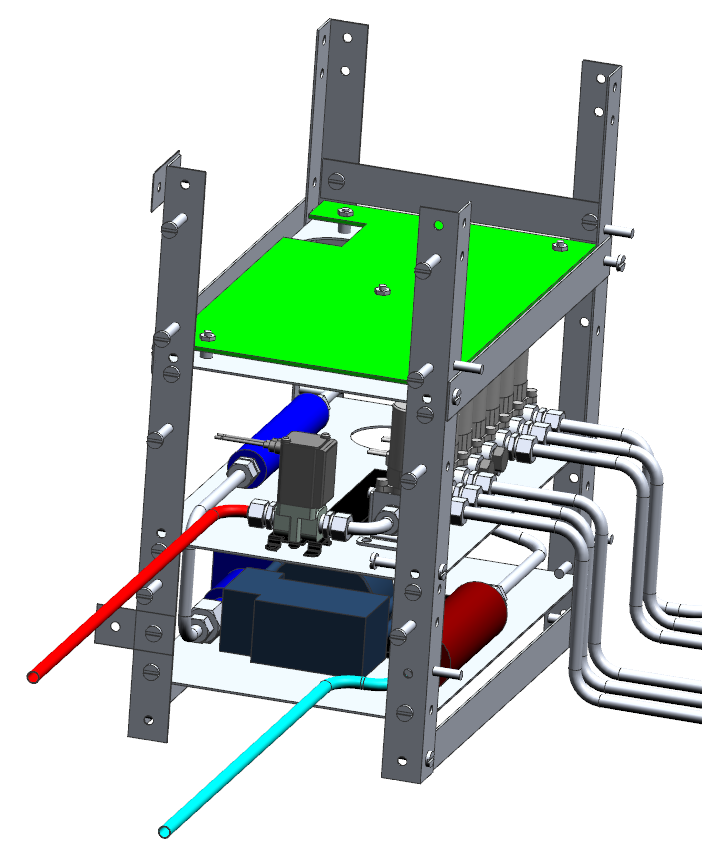
\includegraphics[width=0.8\textwidth]{4-experiment-design/img/Mechanical/Brain_Isometric_Open.png}
    \caption{Isometric View of The Brain without walls.}
    \label{brain_isometric_open}
\end{figure}

Level 1 is the base of the AAC box and together with Level 2 contain the main pneumatic system. This is commanded by the electronics in the top level. This distribution allows easy access to the PCB from the top and provides the physical desired separation between electronics and pneumatic circuit. 

The fact of having different levels implies the need of having dedicated holes to bring all the wires to the third level and the tube to the second level. This is shown in the dedicated section for each level which can be seen in Figure \ref{brain_lateral}.

\begin{figure}[H]
    \centering
    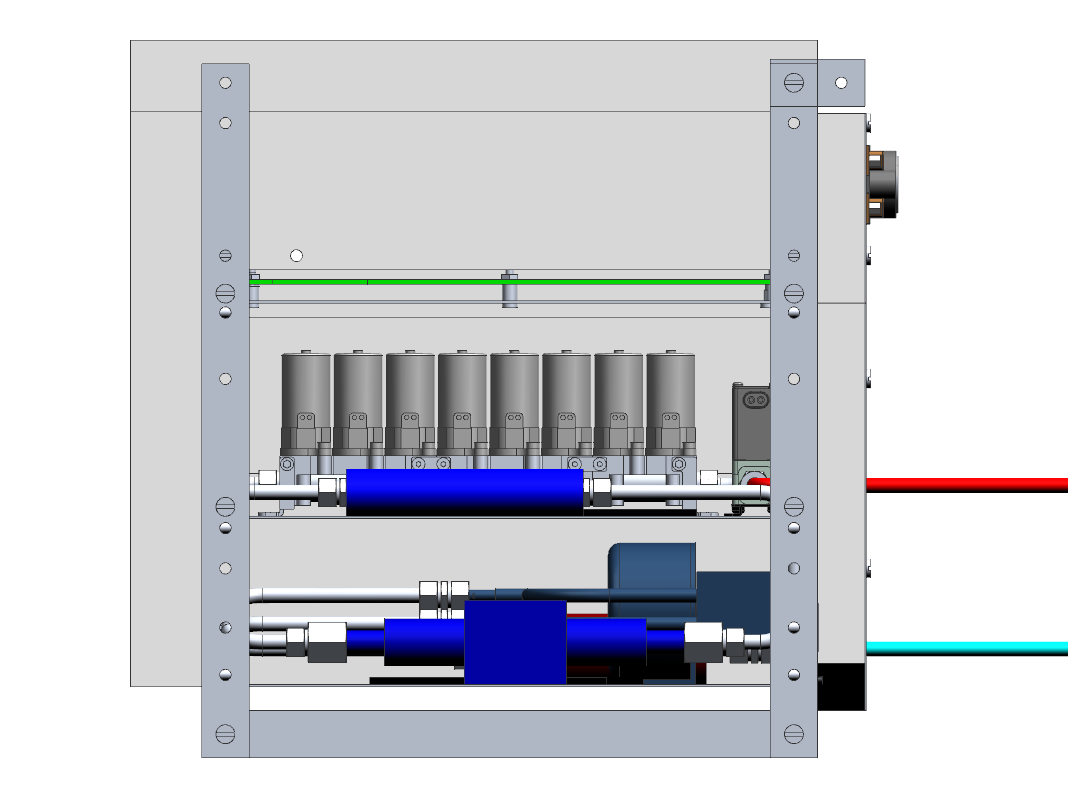
\includegraphics[width=0.8\textwidth]{4-experiment-design/img/Mechanical/Brain_Lateral.png}
    \caption{Lateral View of The Brain.}
    \label{brain_lateral}
\end{figure}

\smallskip
The structure of the Brain provides versatility in terms of implementation and construction. It is made out of four aluminum 90-degree angle bars and five flat bars to join them together. The bars have custom-made holes that allow the 1 mm thick aluminum plate of each level to be fixed by means of two bolts on each column, one over and one below it. They allow the possibility to provide the anchor point for the lateral and top styrofoam shield as well as to fix the whole unit to the box structure bars. This is seen in Figure \ref{brain_structure}. 

\begin{figure}[H]
    \centering
    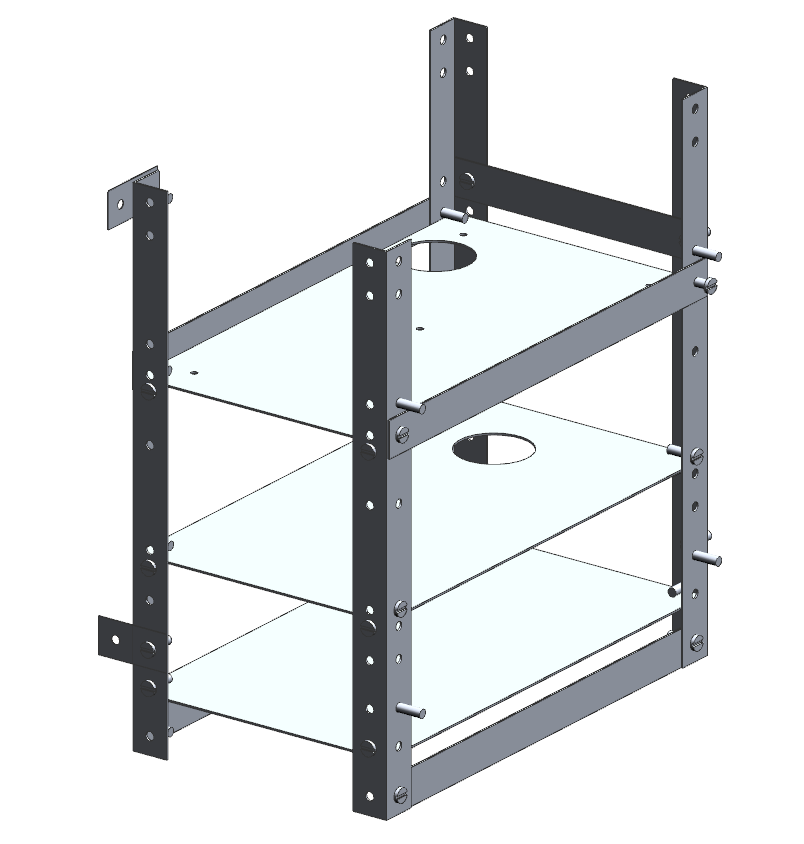
\includegraphics[width=0.8\textwidth]{4-experiment-design/img/Mechanical/Brain_Structure.png}
    \caption{Structure of The Brain.}
    \label{brain_structure}
\end{figure}

\smallskip
The bulk dimensions of the brain are 260 mm long, 150mm wide and 290 mm high. If the shielding styrofoam walls are taken into account, the dimensions are 290 mm long, 180 mm wide and 300 mm high.
Therefore, accounting for the space the column bars take, each plate has a surface of 258 mm x 158 mm. The distance between levels is variable depending on the components dimensions. Level 1 has a height if 7 cm, Level 2 has a height of 9cm and Level 3 has 8cm to the top styrofoam shielding. The Brain with styrofoam sheilding can be seen in Figure \ref{brain_isometric}.

\begin{figure}[H]
    \centering
    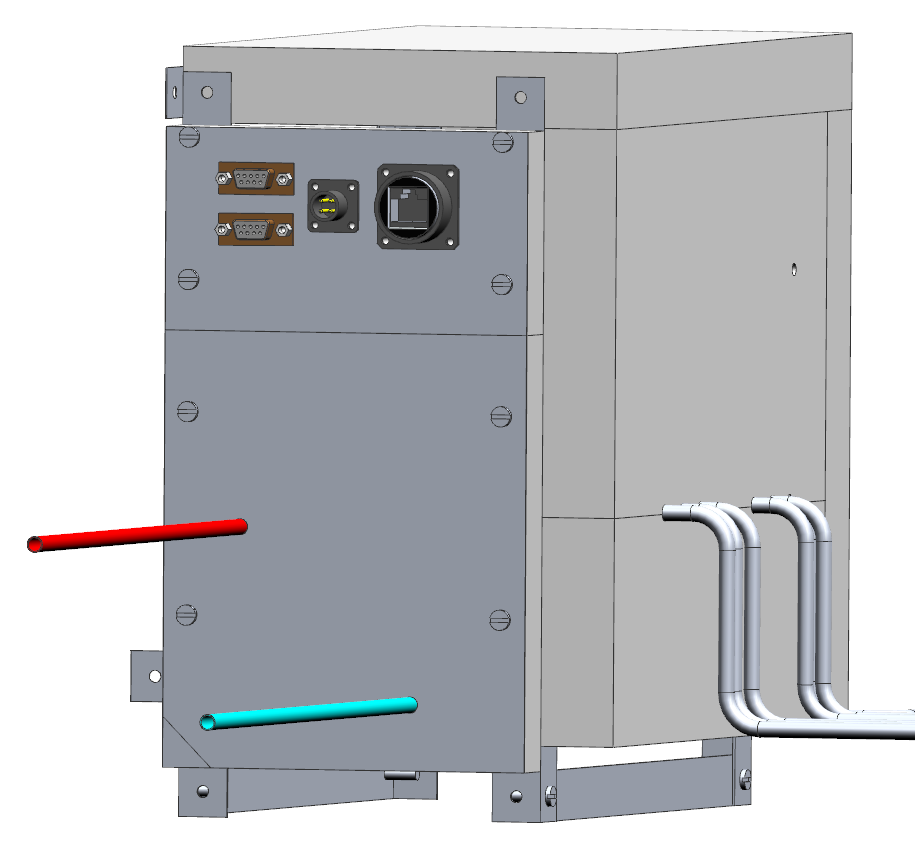
\includegraphics[width=0.8\textwidth]{4-experiment-design/img/Mechanical/Brain_Isometric.png}
    \caption{Isometric View of the Brain.}
    \label{brain_isometric}
\end{figure}

\smallskip
In order to allocate the electrical interfaces required (E-Link, Power Supply and D-Sub Connectors) as well as to allow the tubes of the sampling system to reach the outside environment, the outside facing wall is divided in three pieces. Two small pieces are fixed to the Brain structure. The latter provides easiness of manipulation when having to open the box wall since the little pieces containing the interfaces and the tubes holes, will remain attached. The bottom piece covers Level 1 and 2 while the other, which contains the electrical connections, protects Level 3. These pieces have the same layout as the main wall. 


\pagebreak
\underline{Level 1 - Pump}

\smallskip
List of components of Level 1:

\begin{enumerate}[label=\Alph*.]
    \item 1 Magnesium filter (M48)
    \item 1 Pump (E3)
    \item 1 Airflow sensor (E6)
    \item 1 Temperature sensor (E9)
    \item 2 Heaters (E7)
    \item 4 Tubes (M45)
    \item 3 Straight union interfaces (M41)
    \item 3 Female to tube interfaces (M42)
\end{enumerate}


\begin{figure}[H]
    \centering
    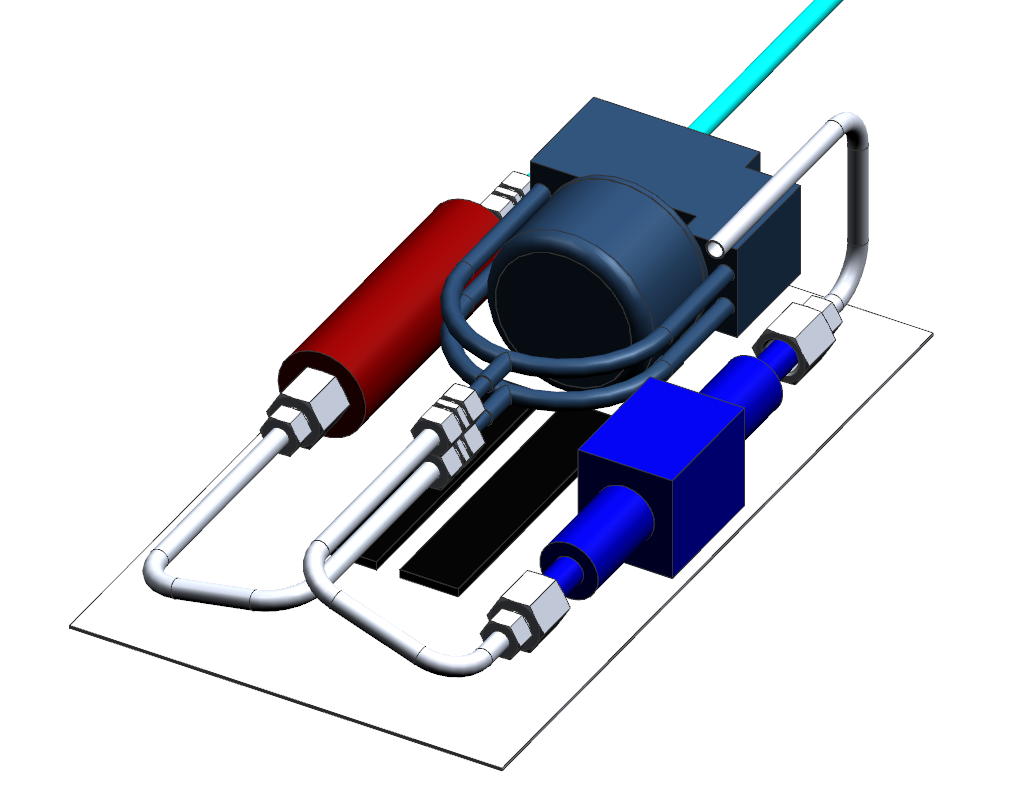
\includegraphics[width=0.8\textwidth]{4-experiment-design/img/Mechanical/Level_1.png}
    \caption{Isometric View of Level 1.}
    \label{level_1}
\end{figure}

\smallskip
The bottom level of The Brain is lying on the base wall styrofoam. It contains the beginning of the pneumatic sampling system. The inlet tube passes through the panel wall and interfaces with the filter. From here the system continues through the pump, airflow sensor and to Level 2.
The reason for having the pump in Level 1 is to have the minimum vibration transmitted to the other components. The pump will have two heaters close by that will be used to regulate its temperature. This can be seen in Figure \ref{level_1}


\pagebreak
\underline{Level 2 - Valve Center}


List of components of Level 2:

\begin{enumerate}[label=\Alph*.]
    \item 1 Sensor Box (M49)
    \item 3 Pressure sensors (E4)
    \item 1 Humidity sensor (E11)
    \item 1 Temperature sensor (E9)
    \item 1 Heater (E7)
    \item 1 Manifold (M50)
    \item 8 Sampling valves (E36)
    \item 1 Flushing valve (E37)
    \item 12 Male to tube interfaces (M40)
    \item 2 Caps (M47)
    \item 12 Tubes (M45)
\end{enumerate}


\begin{figure}[H]
    \centering
    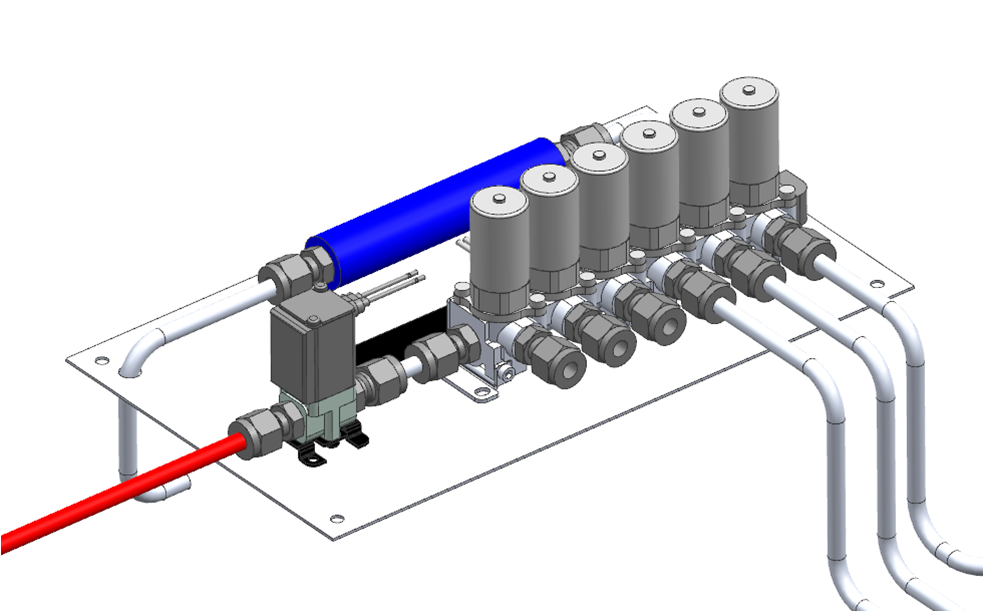
\includegraphics[width=0.8\textwidth]{4-experiment-design/img/Mechanical/Level_2.png}
    \caption{Isometric View of Level 2.}
    \label{level_2}
\end{figure}

\smallskip
This level of the Brain is responsible of the distribution of the air to the selected sampling bag. The manifold with 8 solenoid valves is the main component. From here, the tubes connect with the bags. A T-Union connection is used just before the bag valve. This interface allows the pre-flight flushing of the tubes connecting with the valves as explained previously. 

\smallskip
The flushing valve is the responsible to ensure a proper flushing of the system before each sampling period. From the flushing valve, a the outlet tube (in red) reaches the outside environment. This can be seen in Figure \ref{level_2}.



\pagebreak
\underline{Level 3 - Electronics}


List of components of Level 3:
\begin{enumerate}[label=\Alph*.]
    \item 1 PCB
    \item 2 D-Sub female connectors (E23)
    \item 1 E-link socket (E35)
    \item 1 Power socket (E33)
\end{enumerate}


\begin{figure}[H]
    \centering
    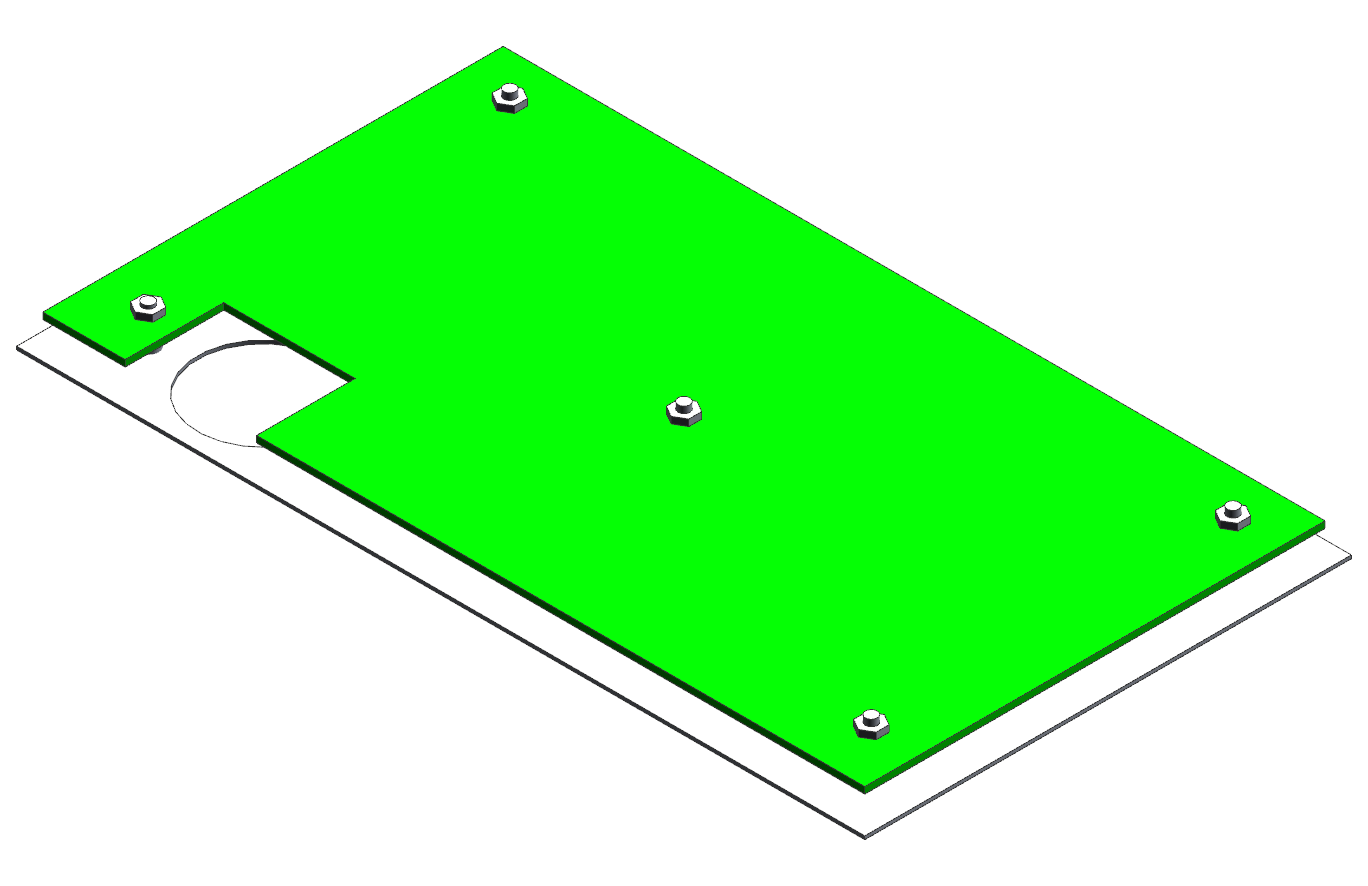
\includegraphics[width=0.8\textwidth]{4-experiment-design/img/Mechanical/Level_3.png}
    \caption{Isometric View of Level 3.}
    \label{level_3}
\end{figure}

\smallskip
The OBC and its external elements will be allocated in the third level of the Brain. The PCB will be fixed to the aluminum plate by means of 5 standoffs. As shown in Figure \ref{level_3}, it has a hole, as well as the level plate, to collect all the wires connecting with levels 1 and 2. This level has its own outside wall which contains the electrical interfaces. The latter allows to open the wall without having to remove all the sockets attached with screws and a female in the inside of the wall. The styrofoam shielding the Brain has a hole at this height to allow the temperature sensors wires to reach the inside of the AAC Box. All the electrical components connected to the PCB in Level 3 are summarized in Tables \ref{tab:list_of_components_CAC} and \ref{tab:list_of_components_AAC}.

\begin{table}[H]
\centering

\begin{tabular}{|l|l|l|}
\hline
\multicolumn{3}{|c|}{\textbf{CAC}}                                                                                      \\ \hline
\multicolumn{1}{|c|}{Area}                        & \multicolumn{1}{c|}{Electrical component} & \multicolumn{1}{c|}{\#} \\ \hline
\rowcolor[HTML]{FFCC67} 
\cellcolor[HTML]{FFCC67}                          & Solenoid valve                            & 1                       \\ \cline{2-3} 
\rowcolor[HTML]{FFCC67} 
\multirow{-2}{*}{\cellcolor[HTML]{FFCC67}CAC} & Temperature sensor                        & 3                       \\ \hline
\end{tabular}
\caption{Connections to CAC Box}
\label{tab:list_of_components_CAC}
\end{table}
\begin{table}[H]
\centering
\begin{tabular}{|l|l|l|}
\hline
\multicolumn{3}{|c|}{\textbf{AAC}}                                                  \\ \hline
\multicolumn{1}{|c|}{Area}                             & Electrical component & \# \\ \hline
\rowcolor[HTML]{FFCCC9} 
\cellcolor[HTML]{FFCCC9}                               & Pump                  & 1  \\ \cline{2-3} 
\rowcolor[HTML]{FFCCC9} 
\cellcolor[HTML]{FFCCC9}                               & Heater                & 2  \\ \cline{2-3} 
\rowcolor[HTML]{FFCCC9} 
\multirow{-4}{*}{\cellcolor[HTML]{FFCCC9}Level 1}     & Temperature sensor    & 1  \\ \hline
\rowcolor[HTML]{9AFF99} 
\cellcolor[HTML]{9AFF99}     & Static Pressure sensor       & 1  \\ 
   \cline{2-3} 
   \rowcolor[HTML]{9AFF99} 
\cellcolor[HTML]{9AFF99}                               & Airflow sensor        & 1  \\ \cline{2-3} 
\rowcolor[HTML]{9AFF99} 
\cellcolor[HTML]{9AFF99}                               & Solenoid valves       & 7  \\ \cline{2-3} 
\rowcolor[HTML]{9AFF99} 
\cellcolor[HTML]{9AFF99}                               & Heater                & 2  \\ \cline{2-3} 
\rowcolor[HTML]{9AFF99} 
\multirow{-5}{*}{\cellcolor[HTML]{9AFF99}Level 2}  & Temperature sensor    & 1  \\ \hline
\rowcolor[HTML]{96FFFB} 
Sampling bags center                                         & Temperature sensor    & 3  \\ \hline
\rowcolor[HTML]{E9D66B} 
Outside                                         & Pressure sensor    & 3  \\ \hline
\end{tabular}
\caption{Connections to AAC System.}
\label{tab:list_of_components_AAC}
\end{table}


\pagebreak
\underline{Shielding and anchor points}

The most critical components in terms of required thermal control are inside the Brain. These are the pump (E3) and the valves (E36 and E37). In order to provide a passive thermal shielding, 3cm thick removable styrofoam walls are placed in the three walls (top and laterals) facing the interior of the AAC box, see Figure \ref{brain_front}. The lateral walls are fixed by means of four bolts attached to the structure bars that penetrate inside the styrofoam. The top wall is fixed in place taking advantage of the structure columns which penetrate inside it. The larger lateral wall, where the tubes from the valves are, is divided in two pieces so it can be removed without having to disconnect the tubes. 

\smallskip
The Brain is fixed to the structure of the AAC box by means of two anchor points. In order to keep it in its place, the structure bars penetrate 3 cm into the styrofoam base.

\begin{figure}[H]
    \centering
    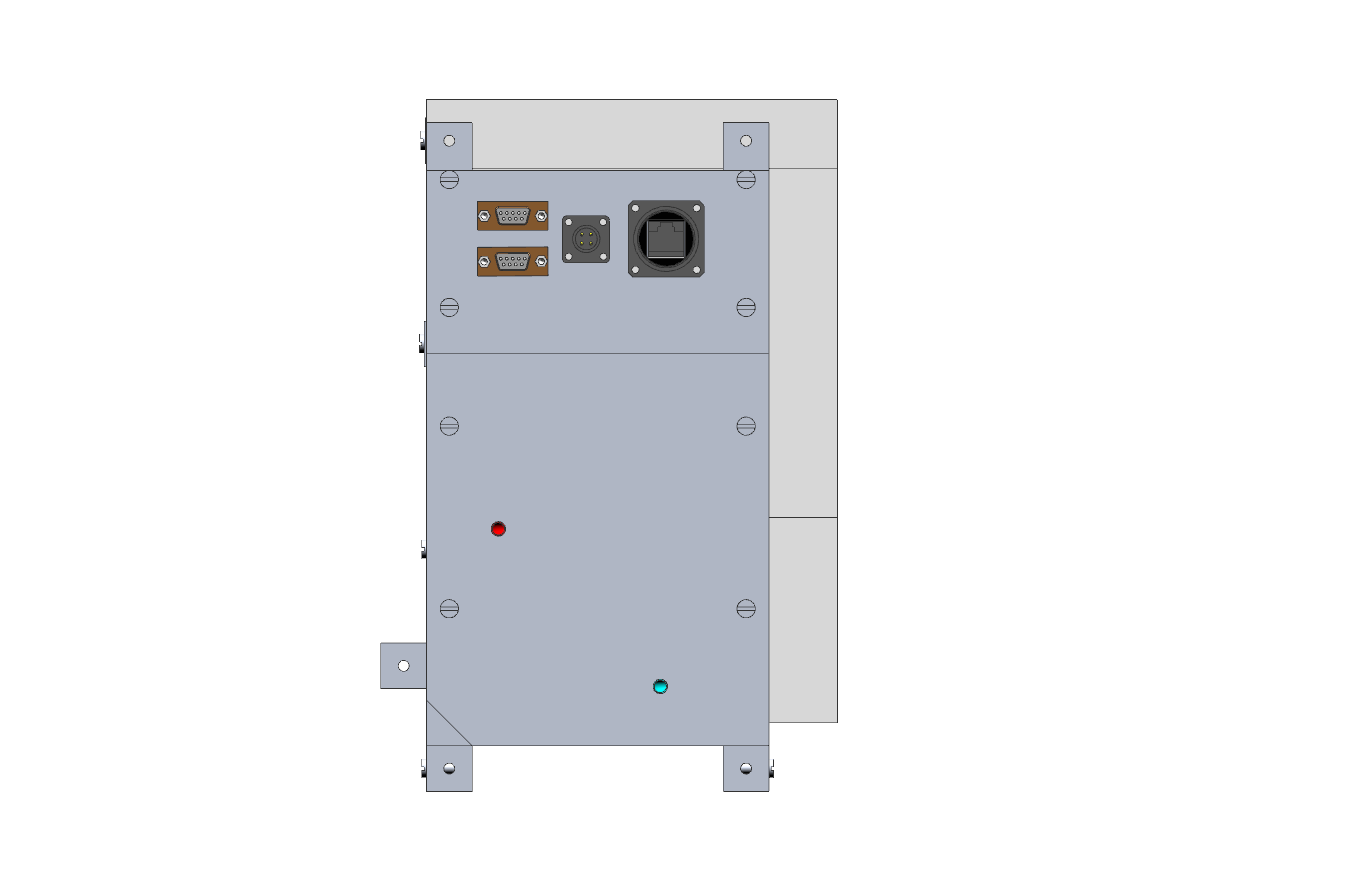
\includegraphics[width=1\textwidth]{4-experiment-design/img/Mechanical/Panel_Front.png}
    \caption{Front View of the Brain Where the Styrofoam Walls can be Identified.}
    \label{brain_front}
\end{figure}


\pagebreak
\subsubsection{Pneumatic System}
\label{sec:4.4.5}

In order to be able to collect separated samples of air, a pneumatic system has been developed. The schematics and components of this can be seen in Figure \ref{pneumatic_system} . The circuit is formed by a total of 81 components located inside the Brain and the AAC Box. 


The schematic for the pneumatic system can be seen in Figure \ref{pneumatic_system}. The air is sucked from the outside through the inlet tube (No.1), turquoise in Figure \ref{level_1_pneumatic_system_top_view}, and it goes through the filter (No.3) inside the pump (No.7). From here, it passes through the airflow sensor (No.11), which allows to monitor the flow rate, before changing to Level 2 (Figure \ref{level_2_pneumatic_system_top_view}). There, the sensor box (No.15) containing three pressure sensors and one humidity sensor, is the first component the air passes through before getting to the 8 stations manifold (No.19). It is in here where the air is directed to the desired bag (No.31) thanks to its dedicated solenoid valve (No.26). 
When flushing the circuitry before each sampling period, the flushing valve (No.23) is opened so the outlet of the system is opened so new air runs through the main circuit. 

\begin{figure}[H]
    \centering
    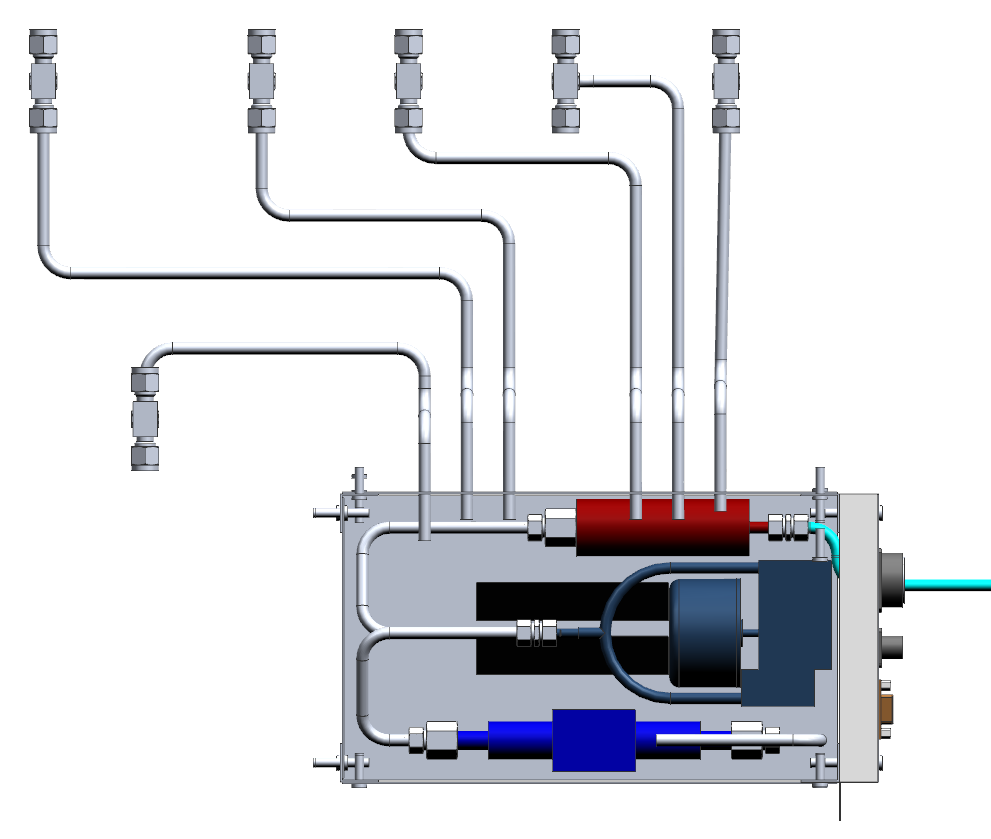
\includegraphics[width=0.8\textwidth]{4-experiment-design/img/Mechanical/Pneumatic_System_Top_View_Level_1.png}
    \caption{Pneumatic System top View of Level 1.}
    \label{level_1_pneumatic_system_top_view}
\end{figure}

\begin{figure}[H]
    \centering
    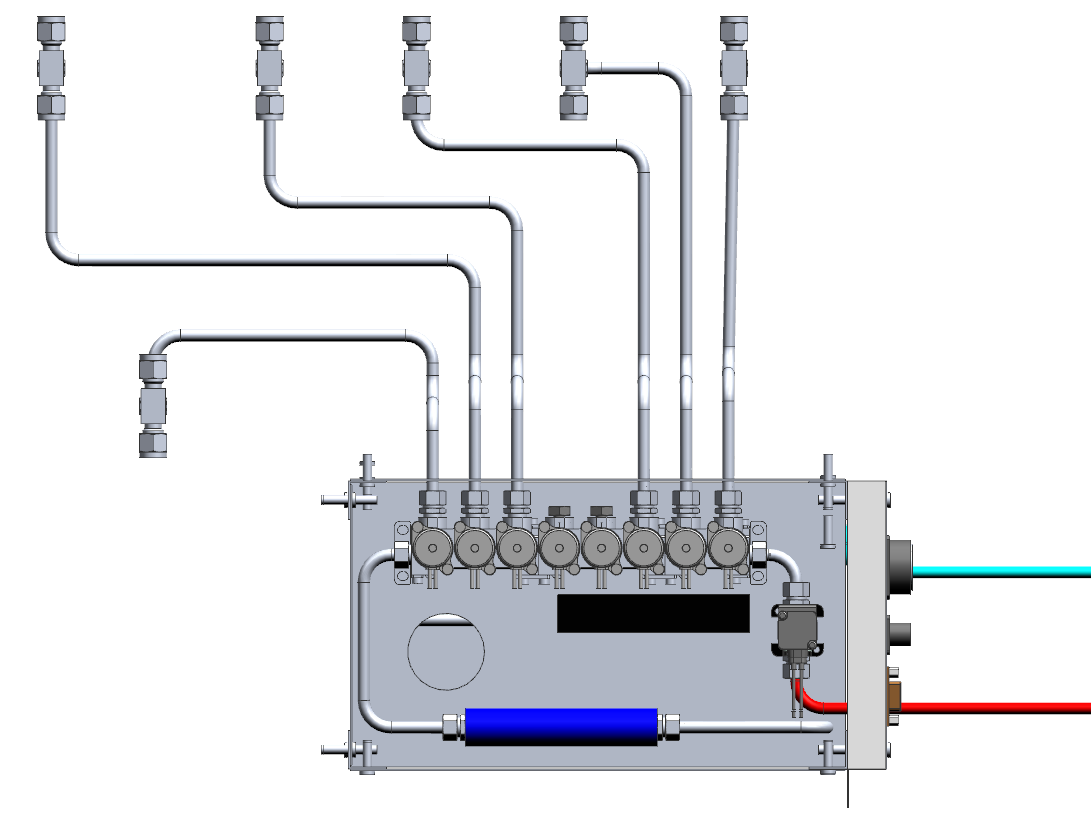
\includegraphics[width=0.8\textwidth]{4-experiment-design/img/Mechanical/Pneumatic_System_Top_View_Level_2.png}
    \caption{Pneumatic System top View of Level 2.}
    \label{level_2_pneumatic_system_top_view}
\end{figure}

% Figure with the diagram

\newpage
\begin{landscape}
\begin{figure}[H]
    \centering
    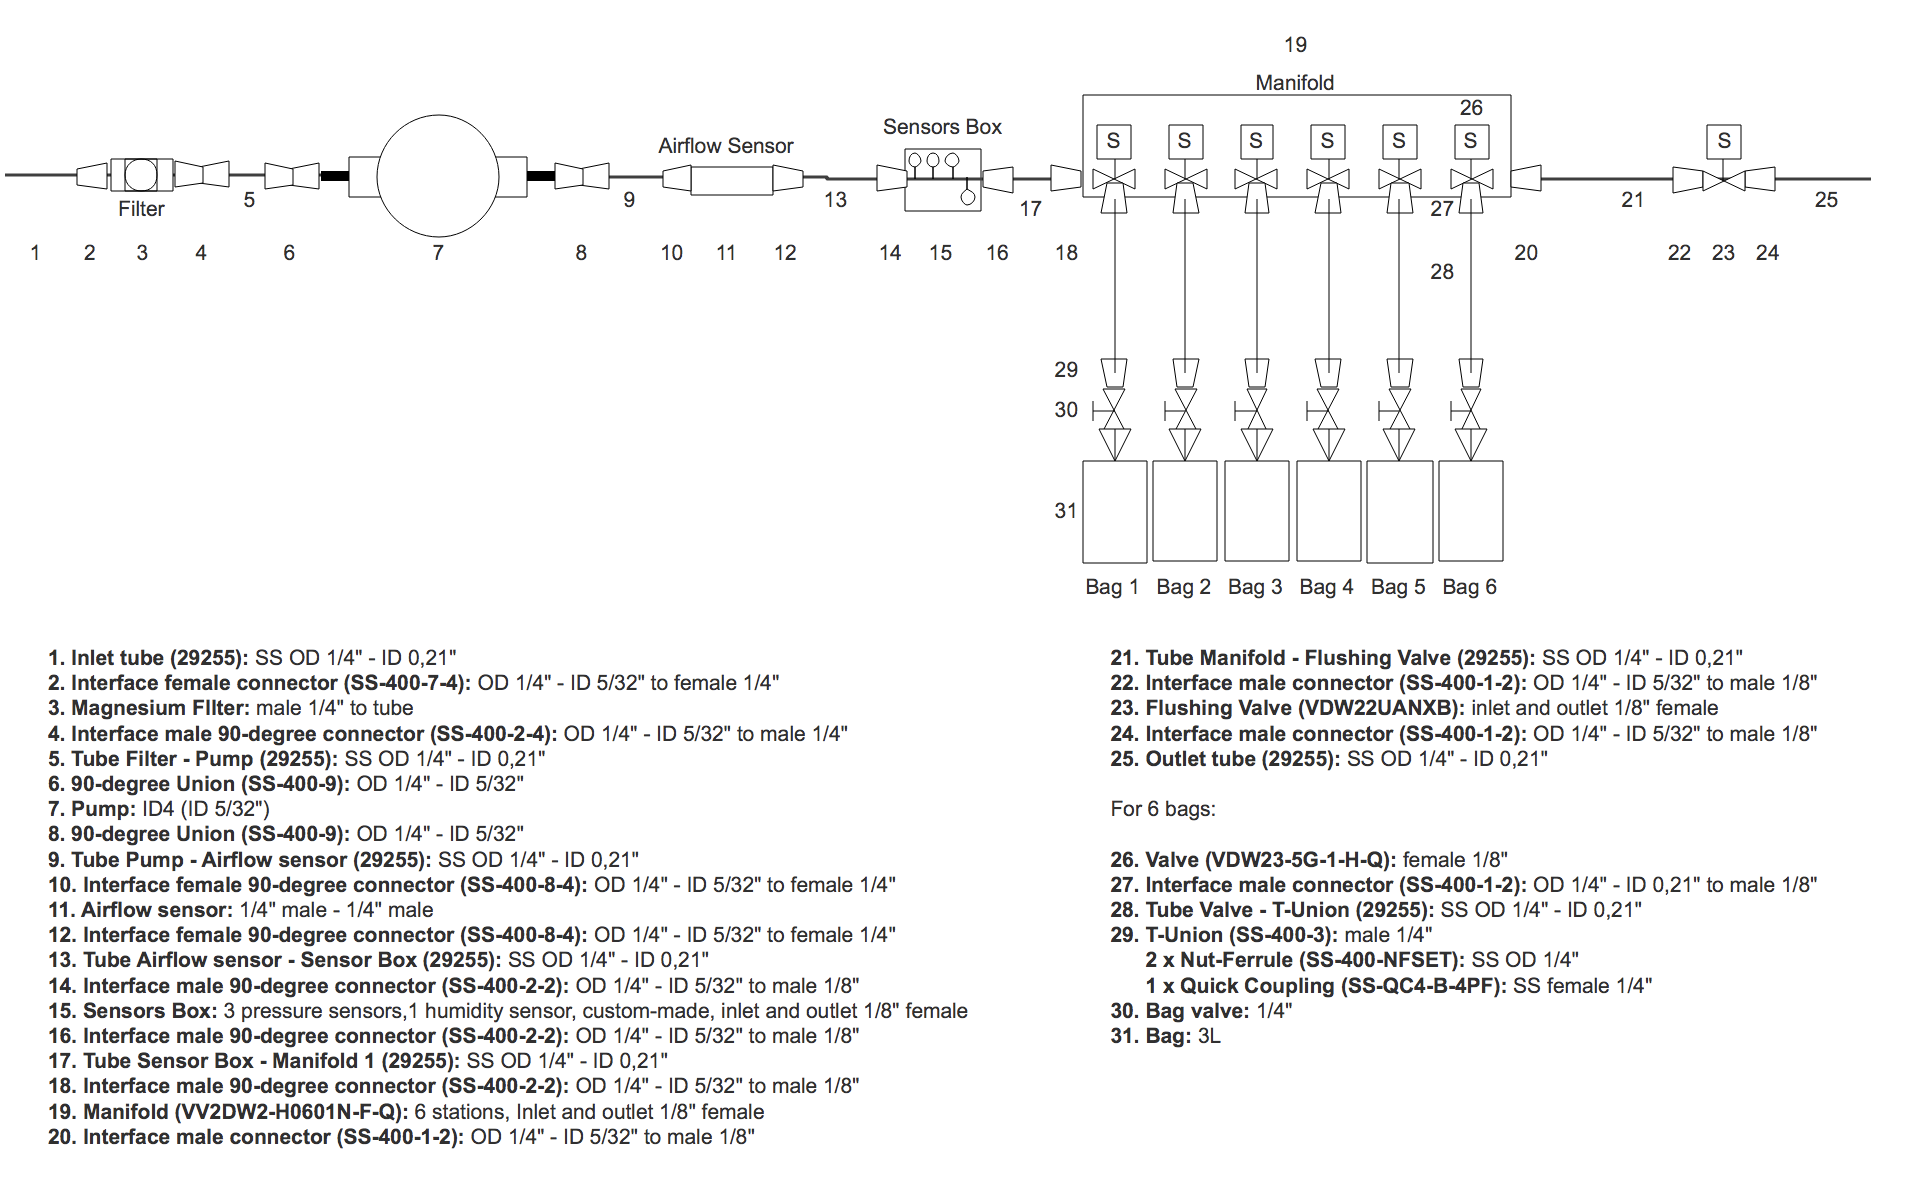
\includegraphics[width=1.5\textwidth]{4-experiment-design/img/Mechanical/AAC_Subsystem.png}
    \caption{AAC Pneumatic System Diagram and Components.}
    \label{pneumatic_system}
\end{figure}
\end{landscape}


\pagebreak
\subsubsection{Protection}

In order to protect the components from all kind of external elements, the experiment box will be shielded with removable aluminum walls along with a thick layer of Styrofoam attached to each wall. No internal space will be lost since the total foam thickness is the same as that of the structural bars in the majority of the walls. 


The walls will protect both the CAC coiled tube and the AAC sampling bags from any external element, unexpected rapid movements, and a probable hard landing impact. %see in Figure \ref{walls}. 
Bolts shall be used to attach all walls to the structure's railed bars. See Section \ref{sec:4.2.1} for detail on fixing points.

%% Figure front wall holes: isometric Include labels

%\begin{figure}[!ht]
%    \centering
%    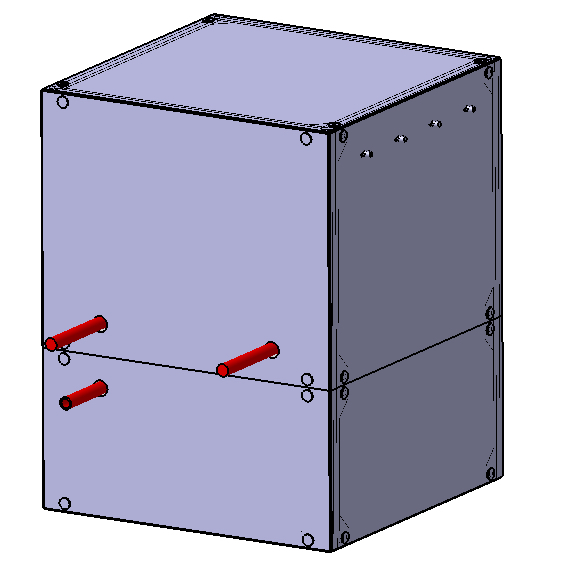
\includegraphics[width=0.7\textwidth]{4-experiment-design/img/frontal_holes.jpg}
%    \caption{External view of the experiment.}
%    \label{front_wall_holes}
%\end{figure}

\raggedbottom